\begin{figure*}[!t]
  \centering
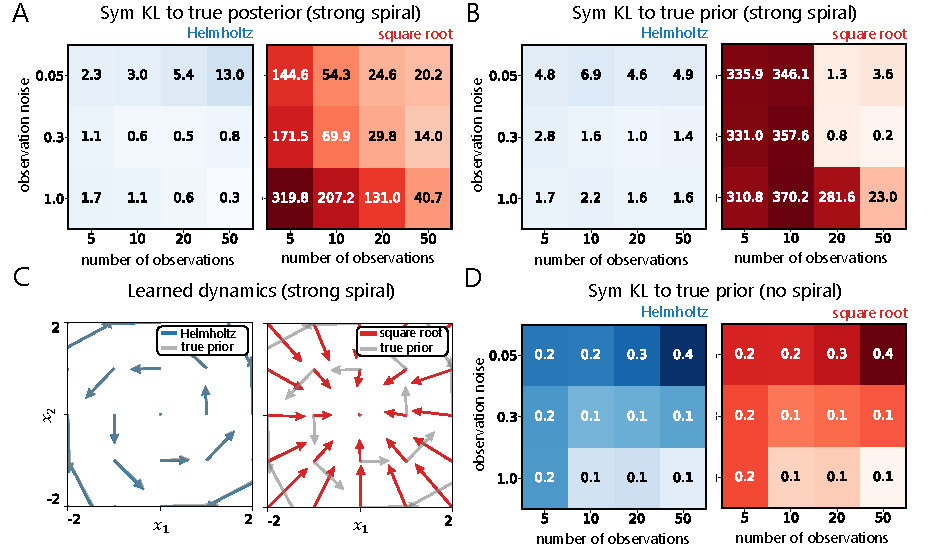
\includegraphics[width=\textwidth]{figs/fig2-spiral-results.pdf}
  \caption{
    Comparison of Helmholtz-SDE and the square root gauge on two OU spiral datasets: strong spiral, $\omega{=}2\pi$ (\textbf{A}-\textbf{C}), and no spiral, $\omega{=}0$ (\textbf{D}). 
    \textbf{A}: The symmetric KL distance (nats) to the posterior across observation noise and number of observations.
    \textbf{B}: The symmetric KL distance to the true prior. 
    \textbf{C}: The dynamics learned by Helmholtz-SDE and the square root gauge against the true prior drift at noise $\sigma = 0.3$ and $N = 10$ observations.
    \textbf{D}: Same as \textbf{B}, but for the no spiral dataset.
  } 
  \label{fig:spiral-results}
  \vspace{-1em}
\end{figure*}

\section{Related Work}

\paragraph{Dynamical systems models.}
Beyond the VI algorithms for latent SDEs discussed in \Cref{sec:background}, several adjacent works model continuous-time, irregularly sampled data. \citet{neklyudov2023action} and \citet{zhang2024trajectory} propose simulation-free methods inspired by score-based generative modeling \cite{hyvarinen2005estimation,songscore2021,lipman2023flow,albergo2025stochastic}, but model the process directly in observation space rather than via a latent SDE. \citet{daemsvariational2024} study latent SDEs driven by fractional Brownian motion. \citet{kiyohara2025neural} develop a VI algorithm permitting simulation-free sampling from both prior and posterior but with a mean-field variational family. A separate line of work replaces the SDE with a latent ODE \cite{heinonen2018learning,chen2018neural,rubanova2019latent,yildiz2019ode2vae}. None of these works address the path-law non-uniqueness arising from marginal-based posterior parameterizations.

\paragraph{Divergence-free constraints.}
Divergence-free vector fields and Helmholtz decompositions appear across machine learning in problems with physical or geometric structure: as parameterizations encoding continuity \cite{richter2022neural} or incompressibility \cite{tompson2017accelerating,li2026project}, and in methods that model or decompose non-gradient vector-field structure \cite{berlinghieri2023gaussian,xu2024hhd,qi2024hdnet,horvatgauge2024,petrovic2025curly}.
Our use is different: rather than imposing a divergence-free condition on the dynamics, we use the Helmholtz decomposition to characterize, at fixed one-time marginals, the family of compatible path laws and the optimal correction to a reference drift.